\section{Microservice Architectures}
% Quick summary of microservice architectures
The \textit{Microservice Architectural Style} has over the last couple of years
gained popularity in development of large scale systems. Inspired by
\textit{Service Oriented Architectures}, but with an increased focus on
services being independent, small, replaceable and limited in responsibilities.
Instead of composing a system of components or libraries, microservice
architectures are composed of small independent services, running in their own
process. They typically communicate through some universal messaging paradigm,
such as \textit{HTTP REST} endpoints or messaging software, such as
\textit{RabbitMQ}.
\\\\
Compared to monolithic architectures which typically group their code in
libraries and layers such as \textit{view}, \textit{business logic} and
\textit{data access}, microservice architectures are split into services that
map to the systems domain. Following \textit{Domain Driven Design} principles
such as \textit{Bounded Context}, each service represents some part of the
domain and communicates with associated parts of the domain through a common
\textit{context}, mapping data to domain concepts. This should ideally result
in a system that is easy to reason about since it mimics the way a specific
domain functions. Grouping associated domain responsibilities in a service,
results in \textit{high cohesion}.
Aligning service development to the domain, results in teams composed of
varying technical capabilities, but builds domain expertise inside a team.
\\\\
Microservice architectures are highly decentralized, and seek to hide internals
of each service to achieve \textit{low coupling} and therefore only integrate
via the chosen communication paradigm. This also means that data-stores are
decentralized. Since a data-store is typically a services internal representation
of state, it is hidden from the outside world and only accessible through the
services interface.
\\\\
Decentralization extends to deployment and environments as well. Microservice
architectures gained traction when operating system level virtualization was
popularized through the open source project \textit{Docker}.
\textit{Docker} utilizes the Linux kernel feature of \textit{Linux Containers},
which allows isolation of processes in a seemingly full-blown operating system.
Linux containers use the hosts operating system kernel and other linux features
such as \textit{cgroups} to create an isolated environment, but with almost no
overhead compared to running processes natively on the OS. 
This achieves per service isolation which is way more efficient compared to typical
hypervisor virtualization and virtual machines, where each environment requires
a full operating system and dedicated slices of the hardware, see
Figure~\ref{fig:hypervisorvscontainer}. Each service hereby has its own
environment, and thinks it runs in its own operating system.
\\\\
\begin{figure}[H]
\centering
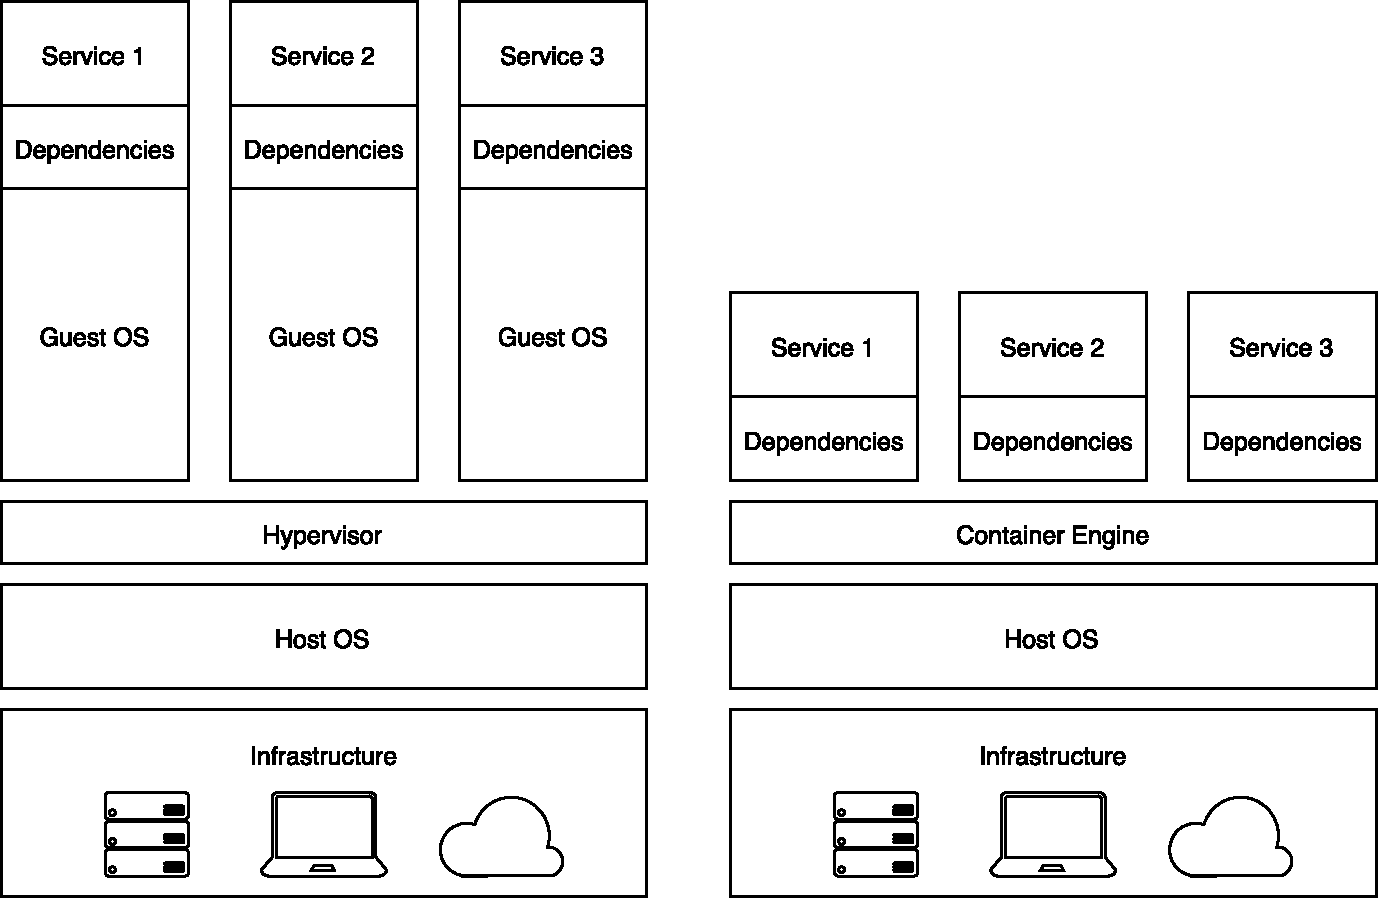
\includegraphics[width=0.8\textwidth]{../media/hypervisorvscontainer.pdf}
\caption{Containers and hypervisor virtual machines differ in the way they 
	virtualize environments and host applications. This visualisation shows that 
	containers have reduced overhead, since a single operating system can run 
	and encapsulate multiple applications, by running them in \textit{Linux} 
	containers. Furthermore they share the resources of the host, instead of 
	having predetermined resources allocated as in virtual machines.}
\label{fig:hypervisorvscontainer}
\end{figure}

Docker functions as a framework to configure, maintain and interact with Linux
containers, and even provides other features such as clustering mechanisms, i.e.\
\textit{Docker Swarm}. \textit{Docker} has defined a common way of describing
the internals of a container, these are called images and are defined in a
\textit{Dockerfile}. These images can be shared on \textit{Docker Hub}.
This project will utilize Linux containers on the \textit{Docker} platform,
across a cluster managed by \textit{Docker Swarm}.
